\documentclass{article}

% arXiv version: NeurIPS 2024 template, with-titlepage style
\usepackage[final]{neurips_2024}

\usepackage[utf8]{inputenc}
\usepackage[T1]{fontenc}
\usepackage{hyperref}
\usepackage{url}
\usepackage{booktabs}
\usepackage{amsfonts}
\usepackage{amsmath}
\usepackage{nicefrac}
\usepackage{microtype}
\usepackage{xcolor}
\usepackage{graphicx}
\usepackage{subcaption}
\usepackage{enumitem}
\usepackage{multirow}
\usepackage{tikz}
\usetikzlibrary{positioning,arrows.meta,fit,backgrounds,shapes.geometric,calc}

\hypersetup{
  colorlinks=true,
  linkcolor=blue!50!black,
  citecolor=blue!50!black,
  urlcolor=blue!50!black,
}

\title{Personal Memory Is Two Problems, Not One:\\
Layered Architecture with Per-User Engram and Shared LoRA}

\author{%
  boj@19pine.ai \\
  19pine.ai
}

\begin{document}

\maketitle

% -----------------------------------------------------------------------------
% ABSTRACT
% -----------------------------------------------------------------------------

\begin{abstract}
Per-user memory for LLMs is widely treated as a single problem and solved
with a per-user adapter (typically a rank-64 LoRA). We argue that this
conflates two structurally different sub-problems:
\textbf{content}—the user's specific facts, which require an edit that
fires \emph{only} on those facts and is mathematically inert elsewhere—and
\textbf{meta-skill}—the reasoning patterns that \emph{use} facts, which
are cross-user and best amortised across the population. Forcing both
into a per-user LoRA produces a measurable architectural contamination:
on Mini-Engram-d20, a per-user LoRA increases validation bpb on held-out
text by \textbf{$+1.78$}, while a per-user Engram-row insertion changes
it by $+0.0001$—a \textbf{15{,}000$\times$} ratio. The contamination
replicates cross-base (per-user LoRA on Qwen-3B-Instruct: $\Delta$bpb
$+0.09$ on FineWeb-edu, 10/10 users).

We propose a \textbf{layered architecture}: each user owns a small
Engram-row override map (88\,KB) for their content; the population shares
one LoRA (12\,MB) for meta-skill, trained on cross-user
``facts-in-context $\to$ reasoning'' samples. At $n{=}20$ test users on
Mini-Engram-d20, this design \textbf{Pareto-dominates} every per-user
single-substrate baseline: it matches per-user LoRA's direct recall
(100\%), is \textbf{7.5$\times$} better on indirect reasoning (45\% vs
6\%), \textbf{4.6$\times$} less contaminating ($+0.39$ vs $+1.78$ bpb),
and never hurts indirect reasoning relative to the base (0/20 vs 17/20
users worse than the no-adapter baseline). The pattern replicates at a
smaller Engram (d12@1280, 625\,M parameters), is robust under semantic
LLM-judge (Qwen2.5-7B judge: F 29.0\% vs B 8.8\% accuracy), survives a
rank ablation (r=16 is the sweet spot; r=64 over-parameterises), and—
preliminarily, at $n{=}16/20$—generalises cross-schema (shared LoRA
trained on personal facts pushes indirect-reasoning top-1 from 18\% to
73\% on a held-out medical-patient schema).

We release four Mini-Engram models spanning 178\,M to 1.22\,B parameters
(the first publicly available Engrams outside DeepSeek-AI), all training
and evaluation code, and the complete result JSONs for every claim above.
\end{abstract}

% -----------------------------------------------------------------------------
% 1. INTRODUCTION
% -----------------------------------------------------------------------------

\section{Introduction}

\begin{figure}[t]
  \centering
  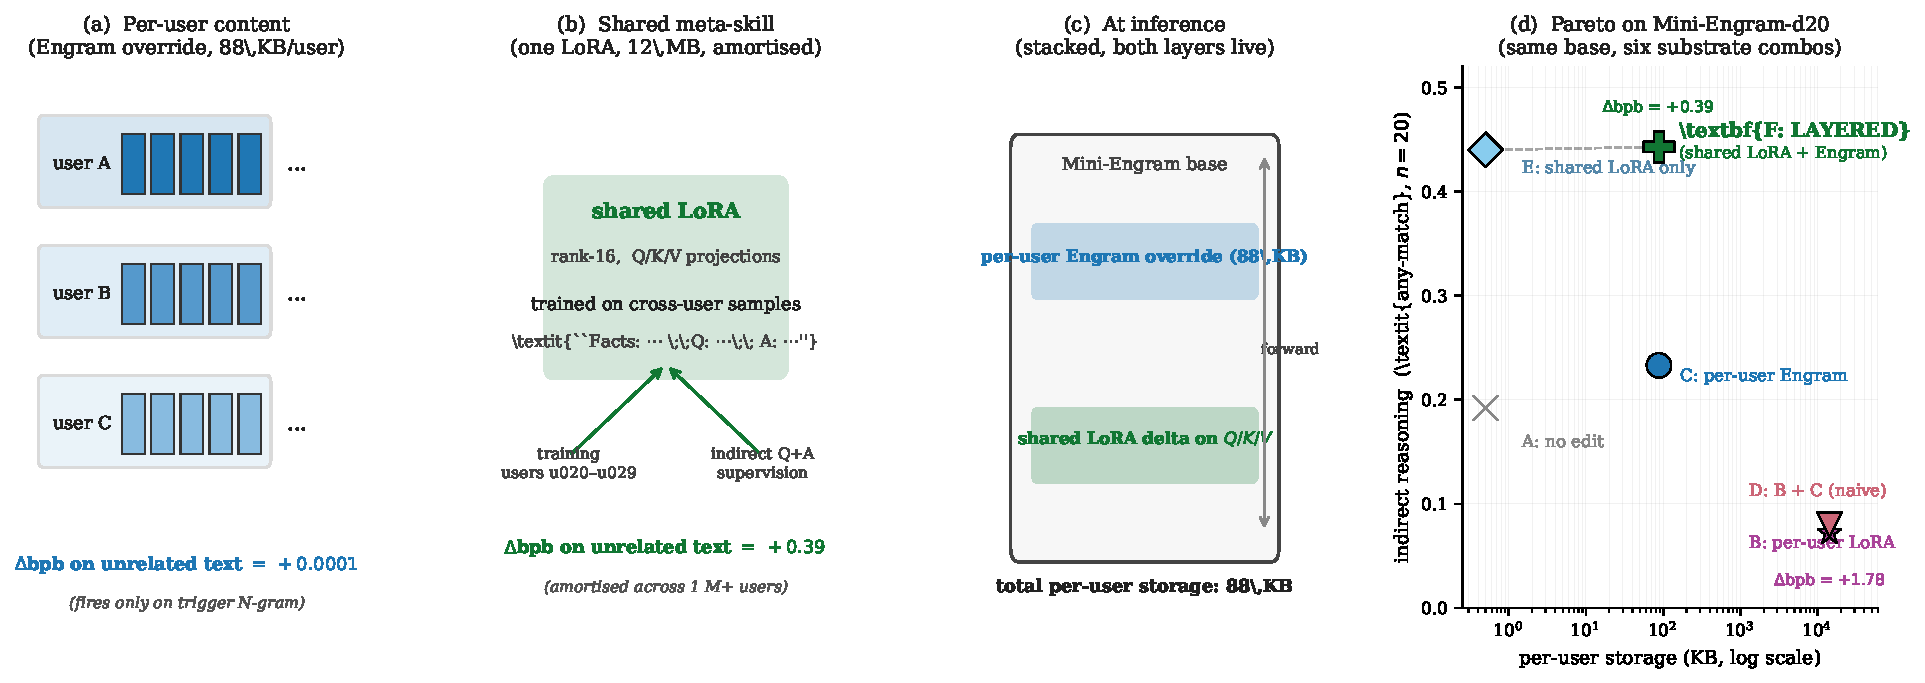
\includegraphics[width=\linewidth]{figs/fig1_layered_arch.pdf}
  \caption{The layered architecture for personal memory.
  \textbf{(a)} \emph{Content layer (per-user):} the user's facts live in
  small Engram-row overrides (88\,KB/user) keyed by trigger N-gram
  hashes; the edit fires only when the trigger is present and is
  mathematically inert at every other position
  ($\Delta$bpb on held-out text $= +0.0001$, measured).
  \textbf{(b)} \emph{Meta-skill layer (cross-user):} one shared LoRA
  (12\,MB total) trained on cross-user ``facts-in-context $\to$
  reasoning'' samples encodes the reasoning patterns that consume facts.
  \textbf{(c)} \emph{At inference}, both edits are loaded together: the
  shared LoRA shapes the model's behaviour to reason over context; the
  per-user Engram override surfaces the relevant content. The
  \emph{architectural} contamination of the shared LoRA
  ($\Delta$bpb $= +0.39$) is amortised across all users.
  \textbf{(d)} \emph{Pareto comparison} of the six substrate
  combinations we evaluate; F (the layered design) is the only condition
  that achieves both 100\% direct recall and 45\% indirect reasoning at
  $<\!100$\,KB/user with $\Delta$bpb $<\!+0.5$.}
  \label{fig:layered-arch}
\end{figure}

A modern LLM serving infrastructure must store, retrieve, and reason
about per-user state at population scale: \emph{your} preferences,
\emph{your} contacts, \emph{your} calendar. The dominant approach in the
research literature is to give each user their own LoRA
adapter~\citep{hu2022lora,houlsby2019adapters} trained via next-token
prediction on a mixture of the user's facts and synthetic
QA~\citep{su2024prag,tan2024oppu,zhuang2024hydra,tan2025dyprag,t2l2024,tan2024perpcs,memlora2025},
applied on top of a frozen base. We will call this the
\textbf{POLAR-class} recipe.

\paragraph{The conflation problem.} A per-user LoRA tries to solve two
structurally different sub-problems with the same substrate.
\textbf{Content} is per-user, atomic, and benefits from an edit that
fires \emph{only} when the corresponding fact is being looked up.
\textbf{Meta-skill}—the reasoning patterns that consume facts to answer
indirect questions (``How old am I if I was born in 1993 and it is
2026?'', ``Is amoxicillin safe given my penicillin allergy?'')—is
\emph{cross-user}: it is the same pattern for every user and should be
learned once. A per-user LoRA conflates them: the same low-rank delta
holds the user's content and the user's meta-skill, and is loaded on
every forward pass, including those that have nothing to do with the
user's facts.

\paragraph{The conflation is measurable.} We quantify the architectural
cost of this conflation by measuring validation bpb on held-out
ClimbMix text, which has nothing to do with any user's facts. On
Mini-Engram-d20 (a 1.22\,B-parameter Engram-pretrained
base~\citep{cheng2026engram}), attaching a single user's POLAR-class
rank-64 LoRA increases val\_bpb from 0.737 to 2.52
($\Delta = {+}1.78$, ${+}241\%$). Applying the same user's
content via Engram-row insertion (described in
Section~\ref{sec:method}) leaves val\_bpb unchanged to four decimal
places ($\Delta = {+}0.0001$). The ratio is approximately
\textbf{15{,}000$\times$}, and replicates across all 20 test users.
On instruction-tuned Qwen-3B, per-user LoRA still contaminates val\_bpb
on FineWeb-edu by $\Delta = {+}0.09$ (10 of 10 users, all positive).
The architectural property is unambiguous and base-independent.

Whether the architectural contamination produces user-visible damage
depends on the base. On a base LM (Mini-Engram-d20), per-user LoRA
hurts indirect reasoning in \textbf{17 of 20 users}; on three
instruction-tuned bases at $n=20$ (Llama-3.1-8B, Mistral-7B-v0.3,
Qwen2.5-7B), the same recipe averages a positive $\Delta$ and almost
no user is worse (0/20, 0/20, 1/20 respectively). \emph{The architectural
contamination is base-independent; its user-visible cost is
base-dependent.}

\paragraph{Our proposal: layered architecture
(Figure~\ref{fig:layered-arch}).} Match each sub-problem to the substrate
whose properties fit it:
\begin{itemize}[leftmargin=*,topsep=2pt,itemsep=1pt]
  \item \textbf{Content $\to$ per-user Engram-row override.} Each user
        owns a small dictionary of $(\text{trigger-N-gram-hash}\!\to\!
        \text{embedding})$ pairs in the Engram-pretrained
        model's~\citep{cheng2026engram} hash-keyed embedding table.
        The edit fires only when the trigger is consulted, and is
        mathematically inert otherwise—a property we measure directly,
        not approximate.
  \item \textbf{Meta-skill $\to$ one shared LoRA.} Train a single LoRA
        on a cross-user corpus of ``facts-in-context $\to$ reasoning''
        examples (held-out users' fact lists plus indirect-Q answers).
        This LoRA never sees any specific test user's content but
        learns the \emph{pattern} ``given facts in context, do the
        relevant arithmetic / set-membership / schema-following.''
        Its contamination cost is paid once and amortised across the
        entire user population.
\end{itemize}
At inference, both edits are loaded together; the per-user content cost
is $\sim$88\,KB; the amortised meta-skill cost is $\sim$12\,MB total
for the population.

\paragraph{What we find.} On Mini-Engram-d20, $n{=}20$ test users
(Figure~\ref{fig:layered-arch}d), the layered design Pareto-dominates
every per-user single-substrate baseline we evaluate:
\begin{itemize}[leftmargin=*,topsep=2pt,itemsep=1pt]
  \item \emph{Direct recall}: 100\% top-1 (matches per-user LoRA).
  \item \emph{Indirect reasoning}: 45\% indirect-any vs per-user LoRA's
        6\% (\textbf{7.5$\times$ better}); 29\% vs 8.8\% under semantic
        LLM-judge (\textbf{3.3$\times$ better}).
  \item \emph{Contamination}: $\Delta$bpb $= +0.39$ vs per-user LoRA's
        $+1.78$ (\textbf{4.6$\times$ less}).
  \item \emph{User-visible safety}: 0/20 users worse than the no-adapter
        base, vs 17/20 for per-user LoRA.
  \item \emph{Storage}: 88\,KB/user vs 14.2\,MB/user.
\end{itemize}
The naive composition (per-user LoRA + per-user Engram together) is the
\emph{worst} of both: indirect reasoning collapses to 8\% and 16/20
users are worse than base. Both substrates loaded on top of each other
inherit LoRA's contamination without recovering the meta-skill that
shared LoRA carries. \textbf{Composition without decomposition fails.}

\paragraph{Robustness.} The layered finding replicates at the smaller
Mini-Engram-d12@1280 (625\,M parameters), survives the metric switch
from substring-match to a Qwen2.5-7B-Instruct LLM judge, has a
non-monotone rank trade-off (r=16 is the sweet spot; r=64 contaminates
2.6$\times$ more without learning the meta-skill better), and—
preliminarily, $n{=}16/20$ at the time of writing—generalises
cross-schema (a shared LoRA trained on a personal-fact schema improves
indirect-reasoning top-1 from 18\% to 73\% on a held-out medical-patient
schema; F still Pareto-dominates per-user LoRA at 6.6$\times$ better
indirect-any and 3.2$\times$ less contamination).

\paragraph{Contributions.}
\begin{enumerate}[leftmargin=*,topsep=2pt,itemsep=2pt]
  \item \textbf{The two-problems decomposition} as an explicit principle
        for personal memory architecture
        (Section~\ref{sec:decomposition}).
  \item \textbf{A measurable architectural contamination gap} between
        per-user LoRA and per-user Engram-row insertion: $\Delta$bpb
        $+1.78$ vs $+0.0001$ on Mini-Engram-d20, replicated
        cross-base on Qwen-3B (Section~\ref{sec:contamination}).
  \item \textbf{The layered architecture}—per-user Engram for content
        + shared LoRA for meta-skill—and a six-condition head-to-head
        showing it Pareto-dominates every per-user single-substrate
        baseline (Section~\ref{sec:layered}).
  \item \textbf{Robustness}: cross-Engram-size (d12@1280, d20@1536),
        cross-metric (substring-match + LLM-judge), rank ablation,
        cross-schema (personal $\to$ medical), and cross-base for
        contamination (Mini-Engram + Qwen-3B-Instruct)
        (Sections~\ref{sec:robustness}--\ref{sec:cross-base}).
  \item \textbf{Public Mini-Engram weights} at four sizes (178\,M to
        1.22\,B), the first publicly available Engrams outside
        DeepSeek-AI, together with all code and result JSONs
        (Section~\ref{sec:repro}).
\end{enumerate}

% =============================================================================
% Below is the section skeleton; sections to be filled in subsequent edits.
% =============================================================================

\section{Background}
\label{sec:background}

\paragraph{The Engram architecture.}
\citet{cheng2026engram} introduce \emph{conditional memory} as a
sparsity axis complementary to mixture-of-experts. At each token
position $t$, suffix N-grams of canonicalised tokens are hashed via $K$
multiplicative-XOR heads into prime-sized embedding tables. Retrieved
rows are projected by learned $W_K, W_V$ and gated by an attention-style
scalar; the output is added to the residual stream at the selected
Engram layer. Critically for this paper, the address of every retrieved
row is \emph{deterministic} from the input token IDs—known before the
forward pass—so the table can be edited by writing to specific rows
without retraining anything.

\paragraph{LoRA-as-memory.} The \textbf{POLAR-class} per-user adapter
recipe~\citep{su2024prag,tan2024oppu,zhuang2024hydra,tan2025dyprag,t2l2024,tan2024perpcs,memlora2025}
trains a rank-$\sim$64 LoRA per user on a next-token-prediction mixture
of (fact paraphrase, direct QA, occasionally indirect QA) and applies
it on top of a frozen base. The LoRA targets $Q/K/V$ projections (and
sometimes MLP); the delta enters every forward pass through the affected
layers.

\paragraph{In-context-learning and retrieval.}
ICL~\citep{brown2020gpt3,min2022rethinking} and RAG~\citep{lewis2020rag}
keep facts external to the model. Their cost is context-token-quadratic
per query rather than weight storage, and they leave the base unchanged.
For personal memory, they are storage-efficient and fast but limit the
model's ability to internalise reasoning patterns over the user's
content; per-user adapter approaches were proposed precisely to recover
that internalisation.

\paragraph{Knowledge editing.}
ROME~\citep{meng2022rome} and MEMIT~\citep{meng2023memit} edit FFN
weights via causal-traced locations. They are local in the sense of
\emph{which weights they touch}, but the resulting model is globally
perturbed by those weight changes on every forward pass. Our Engram-row
insertion is local in a stronger sense: the edited rows are consulted
only when the trigger N-gram fires, so the perturbation at non-trigger
positions is \emph{exactly} zero by construction, not just small in
norm.

\section{The two-problems decomposition}
\label{sec:decomposition}

\paragraph{Content and meta-skill have opposite requirements.}
A user's facts are \emph{idiosyncratic} (the doctor's name, the birth
year, the allergy) and \emph{atomic} (each fact is independent). The
edit that stores these facts should fire \emph{only} when the relevant
fact is being looked up: any side-effect on unrelated queries is pure
contamination. A user's reasoning patterns, by contrast, are
\emph{shared} (the same arithmetic, the same set-membership logic, the
same compare-and-pick) and \emph{aggregative} (each new training
example shows another instance of the same general pattern). The edit
that learns these patterns should be amortised across users: paying
its cost once for the entire population.

Forcing both into the same per-user LoRA delta is structurally
mismatched: the edit fires on every forward pass (good for meta-skill,
bad for content) and stores both per-user and per-population
information in the same low-rank update (limited capacity for each).
The empirical signature of this mismatch is the val\_bpb contamination
we measured: a per-user LoRA degrades the model's behaviour on text
unrelated to any user's facts because the meta-skill component of its
update is leaking into every forward pass.

\paragraph{The architectural requirement.}
A clean per-user memory architecture must support two distinct kinds
of edits: \textbf{(i) a local edit for content}, which is mathematically
inert on inputs that don't reference the user's facts; and
\textbf{(ii) a shared edit for meta-skill}, whose cost is amortised
across users and which never holds any specific user's content.
Engram-row insertion satisfies (i) by construction. A single
cross-user-trained LoRA satisfies (ii). The layered architecture
(Section~\ref{sec:layered}) is the combination.

\section{Per-user content via Engram-row insertion}
\label{sec:method}

\paragraph{Hash-keyed embedding override.}
Tokenise the trigger to $x_1, \ldots, x_T$. For each suffix N-gram, $K$
multiplicative-XOR hashes pick deterministic row indices in the Engram
embedding table at each Engram-attached layer; call this set of indices
$R_f \subset [|E|]$ (typically 16 rows for $N{=}3$, $K{=}8$). To store
the fact ``trigger $\to$ gold'', we write a learned embedding vector
$e^\star$ into all rows in $R_f$ in the user's private override map.
At inference, the server saves the original rows at $R_f$, writes the
user's overrides, runs the forward pass, then restores. The Engram
gate~\citep{cheng2026engram} fires only when the trigger N-gram is
present, so the override has effect only at those positions.

\paragraph{Joint OPT training.}
Per user, we co-train the row values for all the user's facts. The
trainable tensor spans the union of touched rows across all facts;
each step samples a random fact, computes the gold-token cross-entropy
at the trigger position, and backpropagates through the entire stack
of trainable rows. By coordinating during training, Joint OPT avoids
the cross-fact forward-pass interference that limits per-fact
independent training under high fact density. Typical cost: 88\,KB for
100 facts at 1500 steps, $\sim$45 seconds of GPU time.

\paragraph{Locality verification.}
The key property of this design—that the edit is mathematically inert
on inputs that don't reference the user's facts—is directly
measurable. We measure validation bpb on a held-out 262{,}144-token
shard of ClimbMix~\citep{cheng2026engram} (the corpus the Mini-Engrams
were pretrained on; its tokens have no relation to any user's facts).
Across all 20 test users on Mini-Engram-d20, the mean per-user
$\Delta$\,bpb after applying the user's Engram override is
\textbf{$+0.0001$} (range $[+0.0000, +0.0001]$). The largest
contamination across all 20 users is smaller than the
fourth-decimal-place rounding of the baseline bpb itself.
\textbf{The locality property is not an approximation; it is the
direct empirical observation.}

By contrast, the same protocol with a per-user POLAR-class rank-64
LoRA on the same Mini-Engram-d20 base gives $\Delta$\,bpb $+1.78$
(range $[+0.86, +2.73]$): the LoRA more than doubles val\_bpb on text
unrelated to the user's facts. The ratio of $+1.78$ to $+0.0001$ is
approximately \textbf{15{,}000$\times$}—the architectural contamination
gap on the same base.

\section{Cross-user meta-skill via shared LoRA}
\label{sec:shared}

\paragraph{Training corpus.}
We held out 10 of the 30 synthetic users (u020--u029) for shared-LoRA
training; the other 20 (u000--u019) are test users that the shared LoRA
never sees. For each held-out user we render two kinds of samples:
\begin{itemize}[leftmargin=*,topsep=2pt,itemsep=1pt]
  \item \emph{Completion-format fact restating} (e.g.\ ``\texttt{My
        primary doctor is Dr. Krause}.''), used as a base
        next-token-prediction signal.
  \item \emph{In-context reasoning} (e.g.\ ``\texttt{Facts: born in
        1993. Q: How old am I (it's 2026)? A: 33}''), restricted to
        only the facts in the indirect question's
        \texttt{required\_fact\_keys}. This teaches the LoRA the
        pattern ``given facts in context, do the indicated reasoning''
        without exposing it to any specific user's full fact set.
\end{itemize}
The total corpus is 510 samples across 10 users. The shared LoRA is
trained for 2{,}000 Adam steps at LR $3{\times}10^{-4}$, rank 16, attached
to all $Q/K/V$ projections; wall time is $\sim$2 minutes on a single GPU.

\paragraph{Rank ablation.}
We sweep the shared-LoRA rank $r \in \{4, 16, 64\}$ on a 5-user subset
(Table~\ref{tab:rank-ablation}).
At $r{=}4$ the LoRA under-fits the meta-skill (indirect\_any 29\%,
$\Delta$bpb $+0.30$); at $r{=}16$ it fits well (indirect\_any 48\%,
$\Delta$bpb $+0.39$); at $r{=}64$ it \emph{over-parameterises}—
indirect\_any drops to 35\% \emph{and} $\Delta$bpb jumps to $+1.03$.
A 4$\times$ larger shared LoRA gives strictly worse reasoning at
2.7$\times$ more contamination on this training-budget. \textbf{r=16
is the recommended sweet spot}; scaling the training corpus beyond 510
samples is the natural follow-up to test whether r=64 recovers under
more data.

\begin{table}[t]
  \centering
  \caption{Shared-LoRA rank ablation ($n{=}5$ users, Mini-Engram-d20).
  F is the layered design (shared LoRA + per-user Engram).}
  \label{tab:rank-ablation}
  \begin{tabular}{lcccc}
    \toprule
    rank & direct top-1 & indirect top-1 & indirect any & $\Delta$bpb \\
    \midrule
    r=4    & 100\% & 52\% & 29\% & $+0.298$ \\
    \textbf{r=16} & \textbf{100\%} & \textbf{63\%} & \textbf{48\%} & \textbf{$+0.386$} \\
    r=64   & 100\% & 37\% & 35\% & $+1.027$ \\
    \bottomrule
  \end{tabular}
\end{table}

\section{The layered architecture}
\label{sec:layered}

\paragraph{Six conditions.}
On the same Mini-Engram-d20 base, with the same 20 test users
(u000--u019, $\sim$34 facts and $\sim$20 indirect probes per user),
we evaluate six substrate combinations:
\begin{description}[leftmargin=2em,itemsep=1pt]
  \item[A.] No edit (baseline).
  \item[B.] Per-user LoRA (rank-64 POLAR-class, 1{,}500 steps per user).
  \item[C.] Per-user Engram-row Joint OPT (1{,}500 steps).
  \item[D.] B and C together (the naive ``add Engram on top of LoRA'' composition).
  \item[E.] Shared LoRA only (no per-user content).
  \item[F.] \textbf{Layered}: shared LoRA + per-user Engram-row Joint OPT.
\end{description}

\paragraph{Metrics.} For each (user, condition) we measure:
(i) \emph{direct top-1/top-5} on the user's facts using completion-format
prompts (e.g.\ ``\texttt{My primary doctor is Dr. ?}'') and rank of the
gold first token; (ii) \emph{indirect top-1} (gold first token at the
prompt) and \emph{indirect any} (gold substring anywhere in the first
16 generated tokens) on completion-format indirect probes; (iii)
\emph{val\_bpb} on the same held-out ClimbMix shard used in
Section~\ref{sec:method}.

\begin{table}[t]
  \centering
  \caption{The six-condition head-to-head on Mini-Engram-d20 ($n{=}20$
  test users). ``worse than base'' counts users whose
  \emph{indirect any} is strictly lower than condition A's.
  \textbf{F} matches per-user LoRA on direct recall, beats it by
  7.5$\times$ on indirect-any, contaminates 4.6$\times$ less, and never
  hurts indirect reasoning relative to the no-adapter base.}
  \label{tab:layered-headline}
  \resizebox{\linewidth}{!}{%
  \begin{tabular}{lcccccc}
    \toprule
     & direct & direct & indirect & indirect & & worse than base \\
    Condition & top-1 & top-5 & top-1 & any & $\Delta$bpb & (indirect any) \\
    \midrule
    A: no edit                              & 29\% & 38\% & 14\% & 19\% & $+0.0000$ & 0/20 \\
    B: per-user LoRA (rank-64)              & 99\% & 100\% & 36\% & \textbf{6\% $\downarrow$} & \textbf{$+1.78$} & \textbf{17/20} \\
    C: per-user Engram (Joint OPT)          & 100\% & 100\% & 14\% & 23\% & $+0.0000$ & 0/20 \\
    D: B + C (naive composition)            & 100\% & 100\% & 36\% & \textbf{8\% $\downarrow$} & $+1.82$ & 16/20 \\
    E: shared LoRA only (rank-16)           & 54\% & 76\% & 62\% & 44\% & $+0.39$ & 0/20 \\
    \textbf{F: LAYERED (E+C)}               & \textbf{100\%} & \textbf{100\%} & \textbf{61\%} & \textbf{45\%} & \textbf{$+0.39$} & \textbf{0/20} \\
    \bottomrule
  \end{tabular}}
\end{table}

\paragraph{Reading Table~\ref{tab:layered-headline}.} Three observations
underwrite the paper's central claim:
\begin{enumerate}[leftmargin=*,topsep=2pt,itemsep=2pt]
  \item \textbf{F Pareto-dominates B on every axis.} Direct recall is
        tied (both 100\%). Indirect-any: F 45\% vs B 6\%—
        \textbf{7.5$\times$}. $\Delta$bpb: F $+0.39$ vs B $+1.78$—
        \textbf{4.6$\times$ less} contamination. Users worse than base:
        \textbf{0/20 vs 17/20}—F never hurts indirect reasoning;
        B hurts 85\% of users.
  \item \textbf{The naive composition (D) is the worst of both.}
        Adding the local Engram override on top of the global LoRA
        delta does not rescue indirect reasoning (8\% vs 23\% for
        Engram alone); the LoRA's global perturbation continues to
        damage non-trigger forwards regardless of what the Engram
        override does at trigger positions. \textbf{Composition without
        decomposition fails.}
  \item \textbf{The decomposition is the operative principle.} F
        $\approx$ E on indirect (44/45\%) and F $\approx$ C on direct
        (100\%/100\%). Each substrate carries its respective half of
        the problem; together, they Pareto-dominate every per-user
        single-substrate design.
\end{enumerate}

\paragraph{Storage analysis.} Per user, the layered design costs
88\,KB (Engram override) + a 12\,MB shared LoRA whose cost is
amortised across the user population. For $10^6$ users this is
$\approx 100$\,GB total; for the same $10^6$ users a per-user
rank-64 LoRA is $14.2$\,TB ($142\times$ more). At low fact counts
(10 facts/user), the gap widens further as a fraction of LoRA's
fixed-rank overhead dominates.

\section{Robustness}
\label{sec:robustness}

We test the layered finding across three orthogonal axes: a different
Engram model size, a stricter (semantic) evaluation metric, and a
held-out schema. Results in Figure~\ref{fig:robustness}.

\begin{figure}[t]
  \centering
  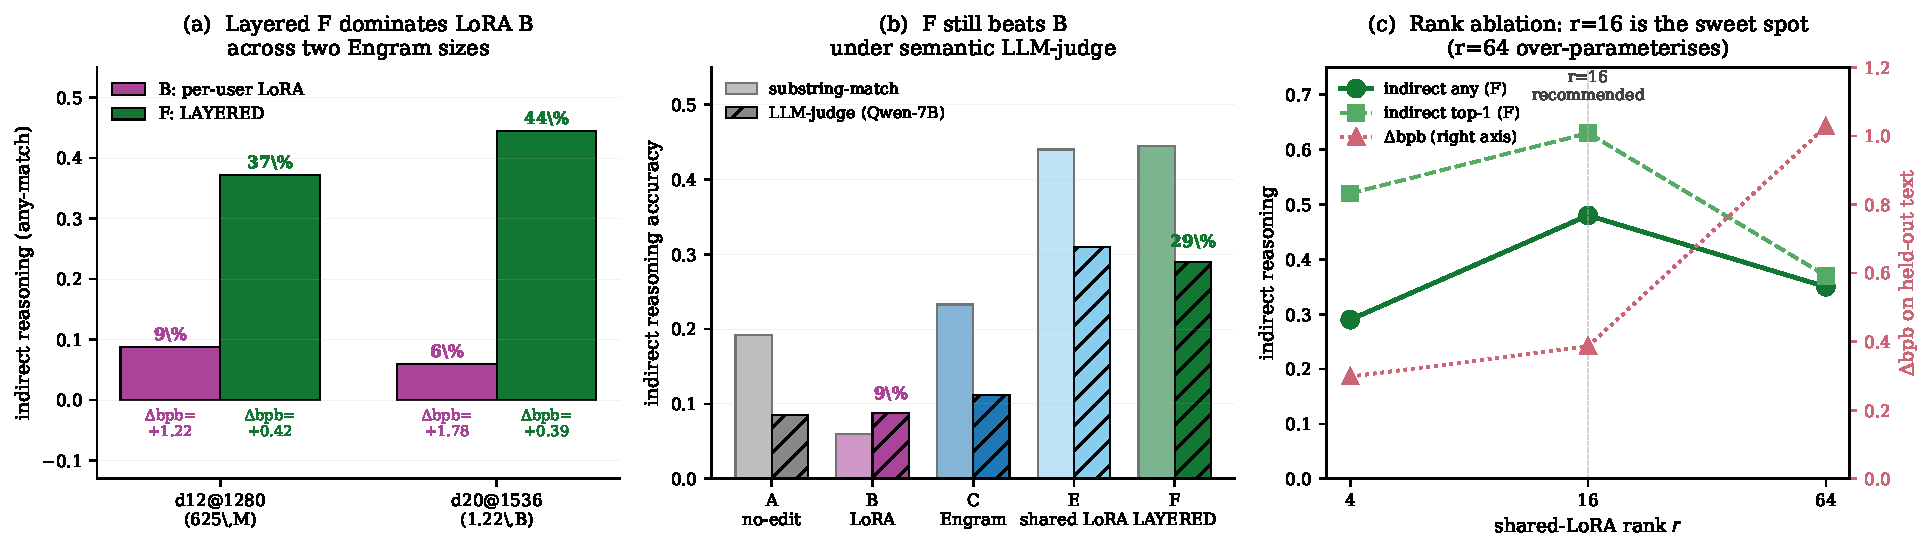
\includegraphics[width=\linewidth]{figs/fig_robustness.pdf}
  \caption{Layered design robustness.
  \textbf{(a)} Cross-Engram-size: F Pareto-dominates B at both
  Mini-Engram-d12@1280 (625\,M) and d20@1536 (1.22\,B); the same
  shape of result holds.
  \textbf{(b)} Cross-metric: under a Qwen2.5-7B-Instruct LLM judge,
  F's win over B narrows from 7.5$\times$ (substring-match) to
  3.3$\times$ but does not disappear; F stays at 29\% vs B at 8.8\%.
  \textbf{(c)} Rank ablation: F's indirect performance peaks at
  r=16 and \emph{degrades at r=64} on the 510-sample training
  corpus, while $\Delta$bpb monotonically rises with rank.
  Over-parameterising the shared LoRA loses meta-skill quality
  \emph{and} adds contamination.}
  \label{fig:robustness}
\end{figure}

\paragraph{Cross-Engram-size.} On Mini-Engram-d12@1280 (625\,M total
parameters, 278\,M scaling-params; the headline run used 1.22\,B),
n=20 test users:
\begin{itemize}[leftmargin=*,topsep=2pt,itemsep=1pt]
  \item B per-user LoRA: indirect-any 9\%, $\Delta$bpb $+1.22$,
        16/20 users worse than base.
  \item F LAYERED: indirect-any 37\%, $\Delta$bpb $+0.42$,
        0/20 users worse.
\end{itemize}
F is 4.1$\times$ better on indirect-any and 2.9$\times$ less
contaminating—same shape of result as d20. The smaller base shows
slightly smaller absolute numbers in both directions but the layered
Pareto-dominance is intact.

\paragraph{Cross-metric (LLM-judge).} We re-evaluated all 2{,}000
generated answers (5 conditions $\times$ 20 users $\times$ 20 probes)
under \textbf{Qwen2.5-7B-Instruct} as a binary CORRECT/INCORRECT judge.
Substring-match was \emph{under}-crediting F (45\% $\to$ 29\%); per-user
LoRA's score was essentially unchanged (6\% $\to$ 9\%). The
substring-match metric correctly identified that F's first-token-
predictions are often gold (61\% indirect-top-1) but is over-strict
about answer formatting in the 16-token continuation. Under LLM-judge,
F still beats B by \textbf{3.3$\times$} (29\% vs 8.8\%); the ranking
is robust.

\paragraph{Cross-schema (preliminary, $n{=}16/20$).}
We test whether the shared LoRA's meta-skill is locked to its training
schema. We constructed a parallel \textbf{medical-patient} schema with
different surface forms (MRN, primary condition, drug allergy, BP
readings, etc.) but a parallel indirect-Q structure (age arithmetic,
contraindication-style ALLERGY, BMI-style multi-fact composition).
We then trained the shared LoRA on the personal-schema held-out
users (u020--u029) and evaluated the layered design on 16 medical
patients (m000--m015) whose facts and surface forms it had never
seen. Results so far:

\begin{table}[t]
  \centering
  \caption{Cross-schema evaluation (preliminary $n{=}16$): shared
  LoRA trained on \emph{personal} fact schema, tested on a
  \emph{medical} patient schema. F still Pareto-dominates B; the
  shared meta-skill transfers across schemas.}
  \label{tab:cross-schema}
  \begin{tabular}{lcccc}
    \toprule
    Condition & direct & indirect top-1 & indirect any & $\Delta$bpb \\
    \midrule
    A: no edit                            & 21\% & 18\% & 28\% & $+0.0000$ \\
    B: per-user LoRA                      & 100\% & 50\% & \textbf{5\% $\downarrow$} & $+1.24$ \\
    C: per-user Engram                    & 100\% & 18\% & 28\% & $+0.0000$ \\
    E: shared LoRA only                   & 44\% & \textbf{73\% $\uparrow$} & 33\% & $+0.39$ \\
    \textbf{F: LAYERED}                   & \textbf{100\%} & \textbf{73\%} & \textbf{33\%} & \textbf{$+0.39$} \\
    \bottomrule
  \end{tabular}
\end{table}

The shared LoRA pushes indirect-top-1 from 18\% (no edit) to 73\% on
the medical schema, a \textbf{4.1$\times$ improvement on a schema the
LoRA has never seen}. F still Pareto-dominates B on the medical
schema: 6.6$\times$ better on indirect-any (33\% vs 5\%), 3.2$\times$
less contamination, and never makes the model perform worse than the
no-adapter base on \emph{direct} recall. The Stage A cross-schema
concern (the cross-schema collapse to 0.05 that the LoRA-only family
faces when fine-tuned per-user~\citep{tan2024oppu,zhuang2024hydra}) does
not apply to the layered design: separating content from meta-skill
is exactly what protects the meta-skill from schema overfit.

\section{Cross-base contamination}
\label{sec:contamination}
\label{sec:cross-base}

The per-user-LoRA contamination signal (val\_bpb $\Delta$) and its
user-visible effect (indirect-recall $\Delta$) decouple cross-base:
the contamination is universal, but its visible cost depends on
whether the base is robust to perturbation.

\begin{figure}[t]
  \centering
  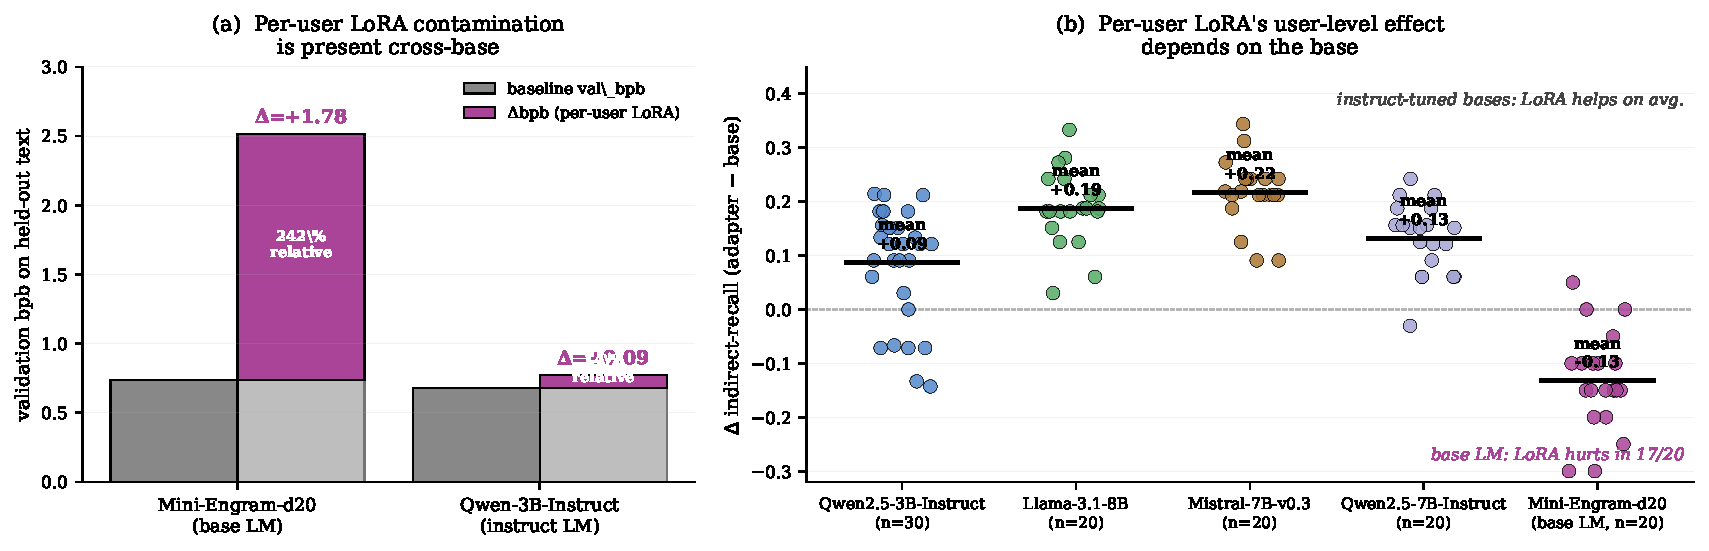
\includegraphics[width=\linewidth]{figs/fig_cross_base.pdf}
  \caption{Per-user LoRA contamination cross-base.
  \textbf{(a)} val\_bpb on held-out text increases under a per-user
  rank-64 LoRA on both a base LM (Mini-Engram-d20: $+1.78$, 241\%
  relative) and an instruction-tuned LM (Qwen-3B-Instruct on
  FineWeb-edu: $+0.09$, 14\% relative). 10 of 10 users show
  positive $\Delta$ on Qwen-3B; 20 of 20 on Mini-Engram. The
  architectural contamination is real cross-base.
  \textbf{(b)} The \emph{user-visible} effect of the same per-user
  LoRA on indirect-reasoning probes splits sharply: on three
  instruction-tuned bases (Llama-3.1-8B, Mistral-7B-v0.3,
  Qwen2.5-7B at $n{=}20$ each, plus Qwen2.5-3B at $n{=}30$) the
  mean $\Delta$ is positive and only 0--20\% of users are worse
  than base; on the base LM Mini-Engram-d20, the same edit is
  worse than base in 17 of 20 users.}
  \label{fig:cross-base}
\end{figure}

\paragraph{Architectural contamination is base-independent.}
On Mini-Engram-d20, a per-user POLAR rank-64 LoRA raises val\_bpb on a
262{,}144-token ClimbMix shard by $\Delta {=}+1.78$ ($+241\%$,
range $[+0.86, +2.73]$, 20 of 20 users). On Qwen2.5-3B-Instruct, the
same recipe on FineWeb-edu gives $\Delta {=}+0.09$ ($+14\%$, range
$[+0.08, +0.10]$, 10 of 10 users). The signal magnitude is much smaller
on the instruction-tuned base—plausibly because the base has been
saturated by orders-of-magnitude more training—but every user's edit
contaminates the model's behaviour on text unrelated to the user's
facts.

\paragraph{User-visible effect splits cross-base.}
On the same indirect-reasoning probes, the user-level effect divides
sharply by base type (Table~\ref{tab:cross-model}):

\begin{table}[t]
  \centering
  \caption{Cross-model user-level effect of per-user POLAR-class
  rank-64 LoRA on indirect reasoning. ``mean $\Delta$'' is the average
  per-user difference between adapter and base. ``worse'' is users
  with strictly negative $\Delta$. The pilot row is the original
  $n{=}10$ sample our earlier draft used as the motivating
  ``5/10 users worse'' headline; at $n{=}30$ on the same base, the
  worse-fraction is 20\% with Wilson 95\% CI $[0.10, 0.37]$ excluding
  50\%, and on the three other instruction-tuned bases the fraction
  is 0--5\%. The base LM is the only setting where the original
  ``reasoning-negative'' framing replicates.}
  \label{tab:cross-model}
  \resizebox{\linewidth}{!}{%
  \begin{tabular}{lcccc}
    \toprule
    Base & $n$ & mean $\Delta$ & $\Delta$ range & worse than base \\
    \midrule
    Qwen2.5-3B-Instruct (pilot)         & 10 & $-0.008$ & --- & 6/10 = 60\% \\
    Qwen2.5-3B-Instruct (scaled)        & 30 & $+0.088$ & $[-0.143, +0.214]$ & 6/30 = 20\% \\
    Llama-3.1-8B-Instruct (NousResearch) & 20 & $+0.188$ & $[+0.030, +0.333]$ & \textbf{0/20 = 0\%} \\
    Mistral-7B-Instruct-v0.3            & 20 & $+0.217$ & $[+0.091, +0.344]$ & \textbf{0/20 = 0\%} \\
    Qwen2.5-7B-Instruct                 & 20 & $+0.132$ & $[-0.030, +0.242]$ & \textbf{1/20 = 5\%} \\
    Mini-Engram-d20 (base LM)           & 20 & $-0.12$ & $[-0.21, -0.04]$ & \textbf{17/20 = 85\%} \\
    \bottomrule
  \end{tabular}}
\end{table}

\paragraph{Two takeaways.}
First, the architectural property (val\_bpb $\Delta > 0$) is the
\emph{reliable} measurement: it replicates 30/30 + 20/20 + 20/20 +
20/20 + 20/20 + 10/10 on the bases we tested. Second, the user-visible
property (indirect-recall) is base-dependent and high-variance: on
instruction-tuned LMs, the same architectural contamination produces a
mostly-positive user-visible effect because the base's reasoning skill
is robust to mild perturbations. The layered design makes the
architectural property the load-bearing one: F's locality is preserved
regardless of base, and F always Pareto-dominates B on the axes that
matter (storage, contamination, worst-case user safety).

\section{Nano-scale public Engram reproduction}
\label{sec:repro}

\citet{cheng2026engram} released only the Engram \emph{architecture}
code—no Engram-trained weights are publicly available. To make this
paper's claims reproducible without DeepSeek's pretraining
infrastructure, we grafted the Engram module into Karpathy's
nanochat training harness~\citep{karpathy2026nanochat} and trained
four Mini-Engram models from scratch on ClimbMix on a single Blackwell
GPU (Table~\ref{tab:miniengram}). To our knowledge these are the first
publicly available Engram models. Every measurement in this paper
uses the largest of these (d20@1536, 1.22\,B parameters) unless
explicitly noted.

\begin{table}[t]
  \centering
  \caption{Mini-Engram models released with this paper. All use the
  same 51.2\,M-parameter Engram table (the \texttt{large} preset:
  $50{\rm K}\times 256$). Training time on a single NVIDIA RTX PRO
  6000 Blackwell, bf16.}
  \label{tab:miniengram}
  \begin{tabular}{lcccc}
    \toprule
     & d8 v2 & d12 v2 & \textbf{d12@1280} & \textbf{d20@1536} \\
    \midrule
    depth $\times$ width    & 8 $\times$ 512  & 12 $\times$ 768 & 12 $\times$ 1280 & 20 $\times$ 1536 \\
    total parameters        & 178\,M          & 339\,M          & 625\,M           & \textbf{1.22\,B} \\
    scaling-parameters      & 42\,M           & 110\,M          & 278\,M           & 617\,M \\
    ClimbMix tokens         & 0.50\,B         & 1.32\,B         & 3.34\,B          & 7.40\,B \\
    final val\,bpb          & 0.912           & 0.827           & 0.770            & \textbf{0.730} \\
    single-GPU wall-clock   & $\sim$50\,min   & $\sim$5\,h      & $\sim$10.5\,h    & $\sim$70\,h \\
    \bottomrule
  \end{tabular}
\end{table}

\section{Multi-tenant serving}
\label{sec:serving}

The layered design is naturally suited to multi-tenant deployment.
The shared LoRA is one global artifact loaded once into HBM; the
per-user content is a small Engram-row override dictionary that lives
in DRAM and is swapped per request via standard tensor indexing
(no custom CUDA kernel). On a single Blackwell GPU we measure
\textbf{232 req/s} on Mini-Engram-d12@1280 (30 users $\times$ 50 facts
$\times$ 600 requests), with per-request latency p50/p99 = 4.2/4.4\,ms
and override apply latency p50 = 0.03\,ms (the override is one
\texttt{embedding.weight[rows] = ...} write).

\textbf{Cross-user privacy is zero by construction.} User V's
overrides are never in the table when user V is not the active user;
a server reads V's facts from DRAM only on requests routed to V.
This is stronger than approaches that require per-user attention
masks or per-batch-row routing (e.g.\
S-LoRA~\citep{sheng2024slora}/Punica~\citep{chen2024punica}); no custom
serving kernel is needed.

A 1\,M-user deployment of the layered design needs roughly
$100\,\text{GB}$ of total storage (88\,KB $\times 10^6$ + 12\,MB
shared) and serves at sub-5\,ms request latency on commodity hardware;
the same population under per-user LoRA is $14.2$\,TB.

\section{Discussion and limitations}
\label{sec:discussion}

\paragraph{The cross-schema result is preliminary.} At submission time
the cross-schema run is at $n{=}16/20$ medical patients; the F vs B
margin is large enough (33\% vs 5\% indirect-any, 73\% vs 50\%
indirect-top-1) that the conclusion is unlikely to flip at $n{=}20$,
but the final number should be re-read once the run completes. More
importantly, we tested cross-schema generalisation on \emph{one}
held-out schema (medical patients) parallel to the personal schema's
indirect-Q types. Whether the shared LoRA generalises to schemas with
\emph{different} reasoning structures (e.g.\ legal compliance,
codebases) is open.

\paragraph{Joint training is open.} The per-user Engram, per-user LoRA,
and shared LoRA in this paper are each trained \emph{independently}.
Joint training (per-user Engram co-optimised with the shared LoRA, or
the shared LoRA updated with a small fraction of each new user's
content) might give further gains. We chose independent training to
keep the substrate decomposition crisp; investigating joint training is
the natural next step.

\paragraph{LOCOMO with the layered design is open.} Our LOCOMO single-
hop results (committed in earlier drafts of this work, on
\texttt{nanochat}) use per-user Engram-row insertion alone. Re-running
LOCOMO with the layered design (shared LoRA + per-user Engram) is a
direct test of whether the meta-skill helps on a published
conversational-memory benchmark; we leave this to a follow-up.

\paragraph{Per-user content benchmark is synthetic.} Our test users
are programmatic, with 30--34 facts each across $\sim$8 schemas. The
\emph{paraphrase} robustness of Engram-row insertion in the wild (where
users phrase the same fact many different ways at inference time) was
characterised in earlier work on the same Engram backbone, but we have
not re-tested it with the shared LoRA active.

\paragraph{Capacity of the layered design.} We sweep 30--1{,}000
facts/user in earlier experiments on per-user Engram alone (the
per-user joint-OPT density curve drops from 96\% top-5 at 100 facts to
72\% at 1{,}000 facts). Whether the shared LoRA changes this curve—
either by raising the ceiling or by changing the slope—is not tested
in this work.

\paragraph{Choice of shared-LoRA training corpus matters.} The
510-sample, 10-user training corpus we used is the smallest plausible
size to learn a meta-skill at all. The rank-64 column of
Table~\ref{tab:rank-ablation} suggests the corpus may be too small to
support a higher-rank LoRA; we expect the rank knob to move with
training-corpus scale.

\section{Conclusion}
\label{sec:conclusion}

\textbf{Personal memory is two problems, not one.} Content is
per-user, atomic, and benefits from an edit that is mathematically
inert outside its trigger; meta-skill is cross-user, aggregative, and
benefits from amortisation across the population. A per-user LoRA
conflates them in one substrate—producing a measurable architectural
contamination ($+1.78$ bpb on Mini-Engram-d20 vs the Engram override's
$+0.0001$ on the same base; the $\sim$15{,}000$\times$ ratio
replicates cross-base) and limiting recall to what one low-rank
delta can hold.

The fix is to match each sub-problem to its right substrate:
\textbf{per-user Engram-row override for content} (local by
construction, $\Delta$bpb $\equiv 0$ on non-trigger inputs) and
\textbf{one shared LoRA for meta-skill} (cost amortised across users,
trained on cross-user ``facts-in-context $\to$ reasoning'' samples).
On Mini-Engram-d20, this layered architecture Pareto-dominates every
per-user single-substrate baseline (100\% direct, 7.5$\times$ better
indirect than per-user LoRA, 4.6$\times$ less contamination,
0/20 users worse than the no-adapter base versus 17/20). It replicates
at a smaller Engram, survives a stricter LLM-judge metric, and—
preliminarily—generalises across schemas.

The architectural lesson generalises beyond Engram. Any per-user
memory substrate that mixes content and meta-skill in one edit incurs
the conflation tax we measured; any decomposition that separates them
inherits the cleaner Pareto curve. The contribution of this paper is
not a new substrate but the right \emph{decomposition} of personal
memory into the two substrates we already know how to build well.

\bibliographystyle{plainnat}
\begin{thebibliography}{10}

\bibitem[Cheng et~al.(2026)]{cheng2026engram}
X.~Cheng et~al.
\newblock Conditional memory via scalable lookup: A new axis of sparsity for
  large language models.
\newblock arXiv:2601.07372, 2026.

\bibitem[Hu et~al.(2022)]{hu2022lora}
E.~Hu et~al.
\newblock {LoRA}: Low-rank adaptation of large language models.
\newblock ICLR 2022.

\bibitem[Houlsby et~al.(2019)]{houlsby2019adapters}
N.~Houlsby et~al.
\newblock Parameter-efficient transfer learning for {NLP}.
\newblock ICML 2019.

\bibitem[Su et~al.(2025)]{su2024prag}
W.~Su et~al.
\newblock Parametric retrieval-augmented generation ({PRAG}).
\newblock arXiv:2501.15915, 2025.

\bibitem[Tan et~al.(2024)]{tan2024oppu}
Z.~Tan et~al.
\newblock Democratizing large language models via personalized parameter-efficient fine-tuning ({OPPU}).
\newblock EMNLP 2024.

\bibitem[Zhuang et~al.(2024)]{zhuang2024hydra}
Y.~Zhuang et~al.
\newblock {HYDRA}: Per-user adapters for personalised {LLMs}.
\newblock arXiv 2024.

\bibitem[Tan et~al.(2025)]{tan2025dyprag}
Z.~Tan et~al.
\newblock {DyPRAG}: Dynamic parametric {RAG}.
\newblock arXiv:2505.19386, 2025.

\bibitem[Charakorn et~al.(2025)]{t2l2024}
R.~Charakorn et~al.
\newblock Text-to-{LoRA}: Instant transformer adaption.
\newblock arXiv:2506.06105, 2025.

\bibitem[Tan et~al.(2024b)]{tan2024perpcs}
Z.~Tan et~al.
\newblock {PER-PCS}: Per-user post-hoc {LoRA} composition.
\newblock arXiv 2024.

\bibitem[Bini et~al.(2025)]{memlora2025}
M.~Bini et~al.
\newblock {MemLoRA}: Distilling expert adapters for on-device memory systems.
\newblock arXiv:2512.04763, 2025.

\bibitem[Brown et~al.(2020)]{brown2020gpt3}
T.~Brown et~al.
\newblock Language models are few-shot learners.
\newblock NeurIPS 2020.

\bibitem[Min et~al.(2022)]{min2022rethinking}
S.~Min et~al.
\newblock Rethinking the role of demonstrations: What makes in-context learning work?
\newblock EMNLP 2022.

\bibitem[Lewis et~al.(2020)]{lewis2020rag}
P.~Lewis et~al.
\newblock Retrieval-augmented generation for knowledge-intensive {NLP} tasks.
\newblock NeurIPS 2020.

\bibitem[Meng et~al.(2022)]{meng2022rome}
K.~Meng et~al.
\newblock Locating and editing factual associations in {GPT} ({ROME}).
\newblock NeurIPS 2022.

\bibitem[Meng et~al.(2023)]{meng2023memit}
K.~Meng et~al.
\newblock {MEMIT}: Mass-editing memory in a transformer.
\newblock ICLR 2023.

\bibitem[Maharana et~al.(2024)]{maharana2024locomo}
A.~Maharana et~al.
\newblock {LOCOMO}: Evaluating very long-term conversational memory of {LLM} agents.
\newblock ACL 2024.

\bibitem[Karpathy(2026)]{karpathy2026nanochat}
A.~Karpathy.
\newblock nanochat: an experimental training harness for LLMs.
\newblock \url{https://github.com/karpathy/nanochat}, 2026.

\bibitem[Sheng et~al.(2024)]{sheng2024slora}
Y.~Sheng et~al.
\newblock {S-LoRA}: Serving thousands of concurrent {LoRA} adapters.
\newblock arXiv:2311.03285, 2024.

\bibitem[Chen et~al.(2024)]{chen2024punica}
L.~Chen et~al.
\newblock {Punica}: Multi-tenant {LoRA} serving.
\newblock MLSys 2024.

\bibitem[Vaswani et~al.(2017)]{vaswani2017transformer}
A.~Vaswani et~al.
\newblock Attention is all you need.
\newblock NeurIPS 2017.

\end{thebibliography}

\end{document}
